\begin{intersong}
    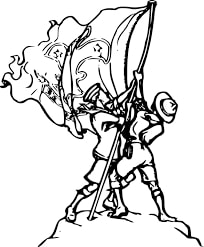
\includegraphics[width=0.4\textwidth]{hetvendel}
\end{intersong}
\beginsong{Het vendel}
\beginverse*
Het vendel moet marsjeren
want Vlaandren is in nood. 
Sint Joris geef ons kleren
geef ons soldij en brood. 
Dat wij geen koude lijden
Geef ons den boer zijn wijf
zijn wolhemd en zijn duiten
dat kan geen zonde zijn. 
\endverse
\beginchorus
Marsjeer, landsknecht marsjeer. 
\endchorus
\beginverse*
Wij slikken stof bij 't wandlen
verstomd zijn lied en lach. 
De keizer slikt heel Vlaandren
hij heeft een sterke maag(d).
Hij denkt al onder 't kauwen
Aan nieuwe roem en eer. 
Thuis weent een blonde vrouwe
als ik niet wederkeer. 
\endverse
\beginverse*
De tamboer slaat de parade
Sint Joris sterke held. 
Bescherm ons in genade
het vendel trekt te veld. 
De pijper wil niet fluiten
wij trekken stil en stom
over de groene heide
opwaarts naar Berg-op-zoom. 
\endverse
\endsong